\documentclass[11pt]{article}
\usepackage[utf8]{inputenc}
\usepackage[shortlabels]{enumitem}
\usepackage{amsmath}
\usepackage{amssymb}
\usepackage{amsthm}
\usepackage{xcolor}
\usepackage{graphicx}
\usepackage{blkarray}

\usepackage{hyperref}
\hypersetup{
    colorlinks=true,
    linkcolor=blue,
    filecolor=magenta,      
    urlcolor=cyan,
}


% setting page format
\topmargin -.5in
\textheight 9in
\oddsidemargin -.25in
\evensidemargin -.25in
\textwidth 7in
\setlength{\parindent}{0 in}
\setlength{\parskip}{0.1 in}

% setting new environments
\newtheorem*{theorem}{Theorem}
\newtheorem*{lemma}{Lemma}
\newtheorem*{corollary}{Corollary}

\theoremstyle{definition}
\newtheorem*{definition}{Definition}
\newtheorem*{example}{Example}
\newtheorem*{problem}{Problem}
\newtheorem*{question}{Question}

\theoremstyle{remark}
\newtheorem*{remark}{Remark}

\newenvironment{solution}[1][Solution]{\textbf{#1:} \par}{\ $\blacksquare$}

\newenvironment{newnotion}[1]{\textbf{#1.}}

\newenvironment{caution}{$\bigstar\bigstar\bigstar$\textbf{Caution.}}

%\newenvironment{proof}[1][Proof]{\textbf{#1:} \par}{\ \rule{0.5em}{0.5em}}
%\newenvironment{problem}[1]{\textbf{#1:} }

% define new commands
\renewcommand{\hat}{\widehat}
\renewcommand{\tilde}{\widetilde}

\newcommand{\numpy}{{\tt numpy}}    % tt font for numpy
\newcommand{\dom}[1]{\mathbf dom #1}
\newcommand{\tr}{\mathbf{tr}}
\newcommand{\sgn}{\text{sgn}}
\newcommand{\spacevert}{\;\vert\;}
\newcommand{\ie}{i.e.}
\newcommand{\eg}{e.g.}

\newcommand{\N}{\mathbb{N}}
\newcommand{\E}{\mathbb{{E}}}
\newcommand{\Q}{\mathbb{Q}}
\newcommand{\R}{\mathbb{R}}
\newcommand{\C}{\mathbb{C}}
\newcommand{\Z}{\mathbb{Z}}
\newcommand{\mS}{\mathbb{S}}

% for probability
\newcommand{\Exp}{\mathbf{E}}
\newcommand{\Var}{\mathbf{Var}}
\newcommand{\Prob}{\mathbf{P}}
\newcommand{\card}{\mathbf{card}}
\newcommand{\cov}{\mathbf{cov}}
\newcommand{\corr}{\mathbf{corr}}
\newcommand{\1}{\mathbf{1}}


% for optimizations
\newcommand{\subto}{\text{s.t.}}

% for norms
\newcommand{\norm}[1]{\left\Vert #1 \right\Vert}
\newcommand{\abs}[1]{\left\vert #1 \right\vert}

\begin{document}
% ========== Edit your name here
\title{MATH 2901 Basic Probability Lecture Notes 3}
\author{Instructor: Richard Kleeman}
\date{}
\maketitle

%\medskip

% ========== Contents begin here ==============
\section{Probability mass functions}
\begin{definition}
The \textbf{(probability) mass function} (p.m.f.) of a discrete random variable $X$ is the function $f: \R \to[0, 1]$ given by $f(x) = \Prob(X = x)$. 
\end{definition}

Notice that $f(x)$ is not discontinuous. The distribution and mass functions are related by
\begin{equation*}
    F(x) = \sum_{i: x_i \leq x} f(x_i), \quad f(x) = F(x) - \lim_{y\uparrow x} F(y).
\end{equation*}

\begin{lemma}
The probability mass function $f: \R \to [0, 1]$ satisfies: 
\begin{enumerate}[(a)]
    \item the set of $x$ such that $f(x) \neq 0$ is \textbf{countable},
    \item $\sum_{i} f(x_i) = 1$, where $x_1, x_2, \dots$ are the values of $x$ such that $f(x)\neq 0$.
\end{enumerate}
\end{lemma}

\begin{example}
\textbf{Binomial distribution.} A coin is tossed $n$ times, and a head turns up each time with probability $p (= 1 - q)$. Then $\Omega = \{H, T\}^n \}$. The total number $X$ of heads takes values in the set $\{0, 1, 2, \dots , n\}$ and is a discrete random variable. Its probability mass function $f(x) = \Prob(X = x)$ satisfies 
\begin{equation*}
    f(k)= \binom{n}{k} p^{k}(1-p)^{n-k}, \quad k=0,1, \ldots, n.
\end{equation*}
The random variable $X$ is said to have the \textbf{binomial distribution} with parameters $n$ and $p$, It is the sum $X = Y_1 + Y_2 + \dots + Y_n$ of $n$ Bernoulli variables.
\end{example}

\begin{example}
\textbf{Poisson distribution.} If a random variable $X$ takes values in the set $\{O, 1, 2, \dots \}$ with mass function
\begin{equation*}
    f(k) = \frac{\lambda^k}{k!} e^{-\lambda}, \quad k = 0, 1, 2, \dots, 
\end{equation*}
where $\lambda > 0$, then $X$ is said to have the \textbf{Poisson distribution} with parameter $\lambda$. Figure \ref{fig:poisson} shows how p.m.f varies with $k$.
\begin{figure}[!htb]
    \centering
    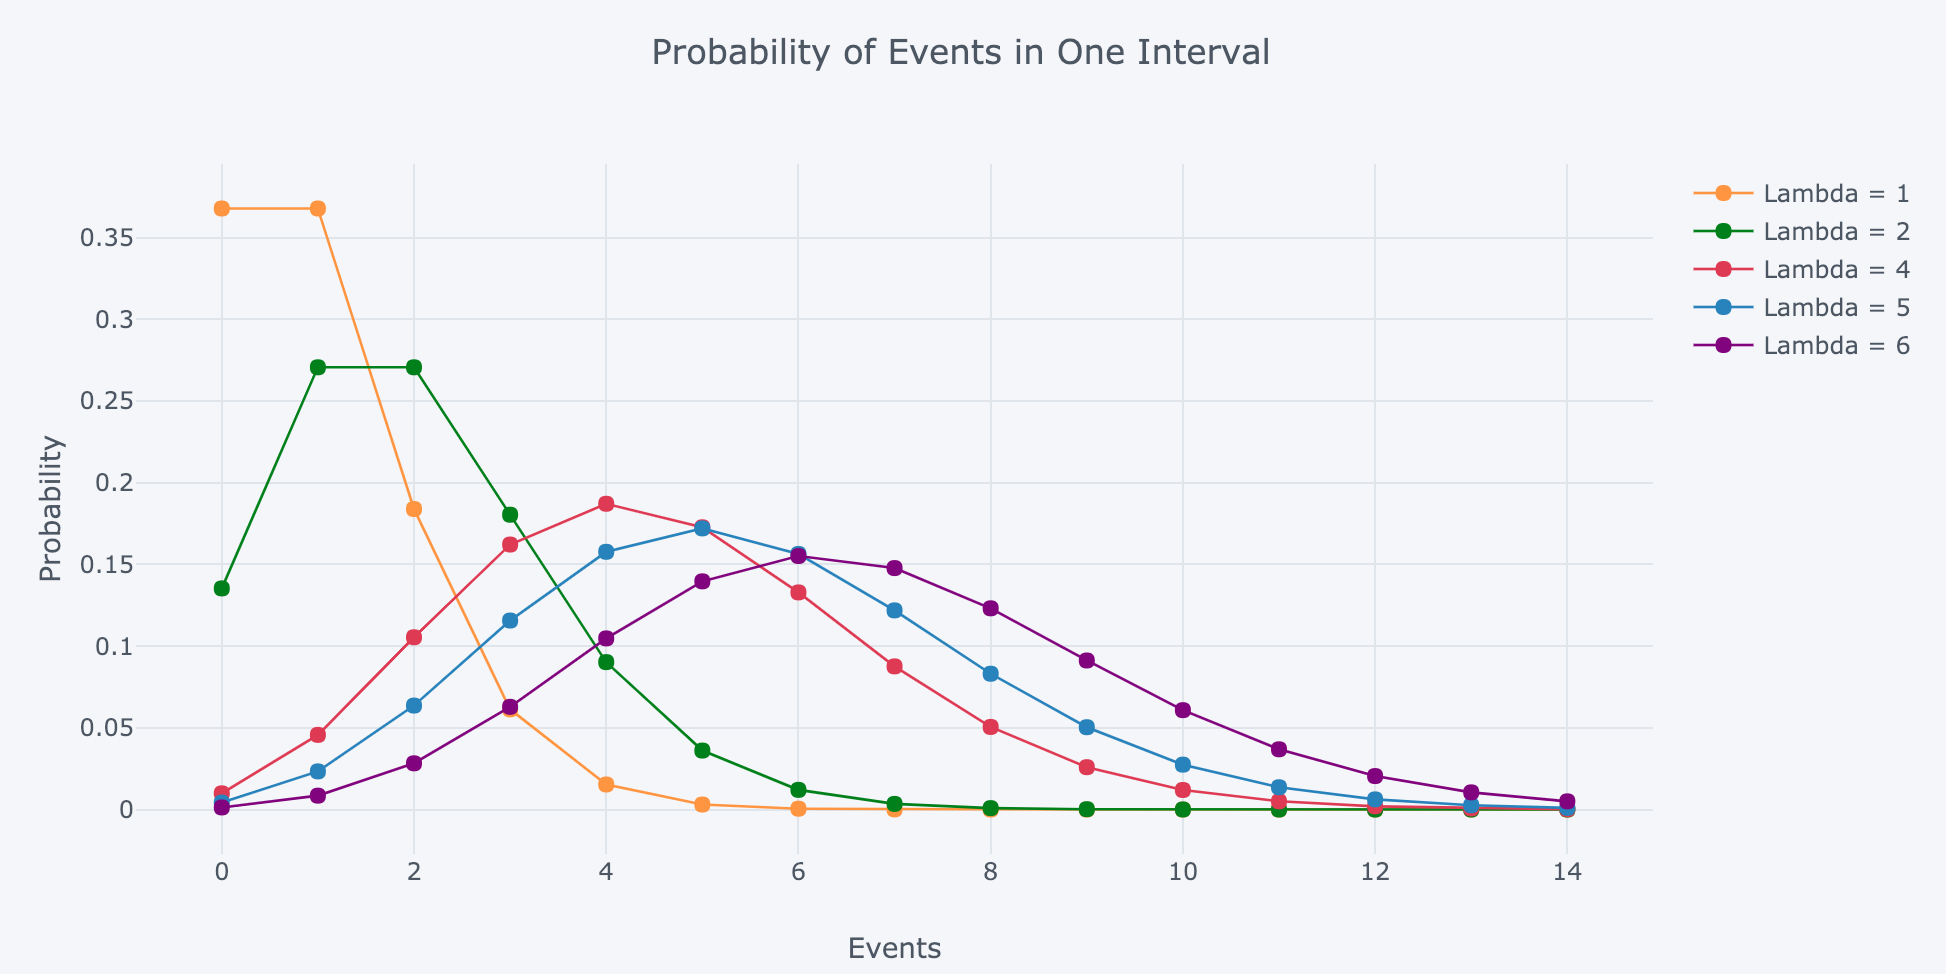
\includegraphics[scale=0.18]{plots/poisson.png}
    \caption{p.m.f of Poisson distribution}
    \label{fig:poisson}
\end{figure}

\begin{remark}
The interpretation of Poisson distribution can be found via this link: \href{https://towardsdatascience.com/the-poisson-distribution-and-poisson-process-explained-4e2cb17d459}{The Poisson Distribution and Poisson Process Explained}.
\end{remark}
\end{example}


\section{Independence of discrete random variables}
Recall that events $A$ and $B$ are called ``independent" if and only if $\Prob(A \cap B) = \Prob(A)\Prob(B)$. 

\begin{definition}
Discrete variables $X$ and $Y$ are \textbf{independent} if the events $\{X = x\}$ and $\{Y = y\}$ are independent for \textbf{all} $x$ and $y$. 
\end{definition}

Let $A: = \{ \omega \spacevert X(\omega) = x \}$ and $B:= \{ \omega \spacevert Y(\omega) = y \}$. Then we can write $P(A) = f_X(x), P(B) = f_Y(y)$ and $P(A \cap B) = f(x, y)$. Therefore, $A$ and $B$ are independent if and only if $f(x,y) = f_X(x) f_Y(y)$ for all $x$ and $y$.

\begin{remark}
The equality $f(x,y) = f_X(x) f_Y(y)$ can be used as the criterion to determine whether two discrete random variables $X$ and $Y$ are independent or not. But \textbf{we need to be careful with it when dealing with continuous random variables} as there will be additional assumptions to determine the independence of continuous random variables using this equality.
\end{remark}

\begin{theorem}
If $X$ and $Y$ are independent and $g, h: \R \to \R$, then $g(X)$ and $h(Y)$ are independent also. 
\end{theorem}

More generally, we say that a family $\{ X_i \spacevert i \in I\}$ of (discrete) random variables is independent if the events $\{X_i = x_i \}, i \in I$, are independent for all possible choices of the set $\{x_i \spacevert i \in I\}$ of the values of the $X_i$ . That is to say, $\{X_i \spacevert i \in I \}$ is an independent family if and only if 
\begin{equation*}
    \Prob(X_i = x_i \text{ for all }i\in J) = \prod_{i\in J} \Prob(X_i = x_i)
\end{equation*}
for all sets $\{x_i \spacevert i \in I\}$ and for all finite subsets $J$ of $I$.


\section{Probability density functions}
Recall that a random variable $X$ is continuous if its distribution function $F(x) = \Prob(X \leq x)$ can be written as\footnote{This is just a general integral, $f(u)$ may or may not be continuous.}
\begin{equation*}
    F(x) = \int_{\infty}^x f(u)du
\end{equation*}
for some integrable $f: \R \to [0, \infty)$.

\begin{definition}
The function $f$ is called the \textbf{(probability) density function} (p.d.f.) of the continuous random variable $X$. 
\end{definition}

\begin{remark}
The function $f$ is \textbf{NOT} unique. We can add some separate points or a countable set of points which has zero measure to $f$. This doesn't change the value of the integral. However, if $F$ is differentiable at $u$ then we shall normally set $f(u) = F'(u)$. 
\end{remark}

Next, we assume $f$ is continuous, then from the basic theorem of calculus, $F$ must be differentiable. Recall 
\begin{equation*}
    P(a < X(\omega) \leq b) = F(b) - F(a) = \int_{a}^b f(u)du.
\end{equation*}
Then $P(X=x) = F(x) - \lim_{y \uparrow x} F(y)$. $F$ is \textbf{absolutely continuous} for continuous random variables. Thus we have
\begin{equation*}
    \lim_{y\uparrow x} F(y) = F(x) \quad \Rightarrow \quad P(X=x) = 0 \quad \forall x\in\R.
\end{equation*}
This means \textbf{the probability of a continuous random variable $X$ taking value at a certain point is 0}. Very roughly speaking, this lies in the observation that there are uncountably many possible values for $X$; this number is so large that the probability of $X$ taking any particular value cannot exceed zero. 

The numerical value $f(x)$ is \textbf{NOT} a probability. Check the probability $\Prob(x < X \leq x + dx)$ for a very small $dx$:
\begin{equation*}
    \Prob(x < X \leq x + dx) = F(x + dx) - F(x) \approx f(x) dx. 
\end{equation*}
Since $dx$ is a very small interval rather a number, we cannot say $f(x)$ is the probability of something.

\begin{lemma}
If $X$ has density function $f$, then
\begin{enumerate}[(a)]
    \item $\int_{-\infty}^\infty f(x)dx = 1$,
    \item $\Prob(X=x) = 0$ for all $x \in \R$,
    \item $\Prob(a < X \leq b) = \int_a^b f(x)dx$.
\end{enumerate}
\end{lemma}

\section{Independence of continuous random variables}
\subsection{Independence of general random variables}
\begin{definition}
Random variables $X$ and $Y$ are called \textbf{independent} if $\{ X \leq x\}$ and $\{Y \leq y\}$ are independent events for all $x, y \in \R$. 
\end{definition}
Note that this definition is the \textbf{general} definition of the independence of any two variables $X$ and $Y$, \textbf{regardless of their types}. The independence of discrete random variables is included in this definition. 

Recall the marginalization. If two random variables $X$ and $Y$ are independent, we have
\begin{equation*}
    \Prob(X\leq x) = \lim_{y\to\infty}F(x, y) \equiv F_X(x), \quad 
    \Prob(Y \leq y) = \lim_{x\to\infty}F(x, y) \equiv F_Y(y).
\end{equation*}
Therefore,
\begin{equation}
    \label{eq:*}
    \tag{*}
    F(x,y) = \Prob(X \leq x, Y \leq y) = \Prob(X\leq x) \Prob(Y \leq y) = F_X(x) F_Y(y). 
\end{equation}
Note that we are dealing with distribution function in \eqref{eq:*}. \eqref{eq:*} can be used as the general criterion to determine whether two random variables are independent or not.

\subsection{Independence of continuous variables}
If $X, Y$ are continuous, then we have
\begin{equation*}
    F(x, y) = \int_{-\infty}^x \int_{-\infty}^y f(x,y) dx dy.
\end{equation*}
\begin{equation*}
    F_X(x) = \int_{-\infty}^x \int_{-\infty}^\infty f(x, y)dx dy \quad \Rightarrow \quad f_X(x) = \int_{-\infty}^\infty f(x,y)dy,
\end{equation*}
where $f_X(x)$ is called the \textbf{marginal probability density function} of $X$. Similarly, we can define $F_Y(y)$ and $f_Y(y)$.

Assume $f(x,y)$ is continuous, then $F(x,y)$ must be twice differentiable w.r.t. $x$ and $y$. Therefore, from \eqref{eq:*}, we can derive a \emph{very practical criterion} to determine the independence of two continuous random variables:
\begin{equation}
    \label{eq:**}
    \tag{**}
    f(x,y) = \frac{\partial^2 F(x,y)}{\partial x \partial y} = \frac{\partial}{\partial x \partial y} F_X(x) F_Y(y) = f_X(x) f_Y(y).
\end{equation}

\begin{remark}
Note that the prerequisite of \eqref{eq:**} is that \textbf{$f(x,y)$ is continuous}.
\end{remark}

\begin{example}
\textbf{Uniform distribution.} The random variable $X$ is uniform on $[a, b]$ if it has distribution function
\begin{equation*}
    F(x) = \begin{cases} 
        0 & x \leq x, \\ \frac{x-a}{b-a} & a < x \leq b, \\ 1 & x > b
    \end{cases}.
\end{equation*}
The density function is
\begin{equation*}
    f(x) = \begin{cases} \frac{1}{b-a} & a < x \leq b \\ 0 & o.w. \end{cases}
\end{equation*}
\end{example}

\begin{example}
\textbf{Exponential distribution}. The random variable $X$ is exponential with parameter $\lambda(> 0)$ if it has distribution function 
\begin{equation*}
    F(x) = 1 - e^{-\lambda x}, \quad x \geq 0.
\end{equation*}
The density function is
\begin{equation*}
    f(x) = \begin{cases} \lambda e^{-\lambda x} & x > 0 \\ 0 & o.w.
    \end{cases}
\end{equation*}
Note that $F(x)$ is not differentiable at $x=0$. This means $f$ has discontinuity at $x=0$. Thus we need to choose some value for $f(0)$. It doesn't matter what value we choose as it doesn't affect the integral. Figure \ref{fig:exponential} shows the p.d.f. of Exponential distribution.
\begin{figure}[!htb]
    \centering
    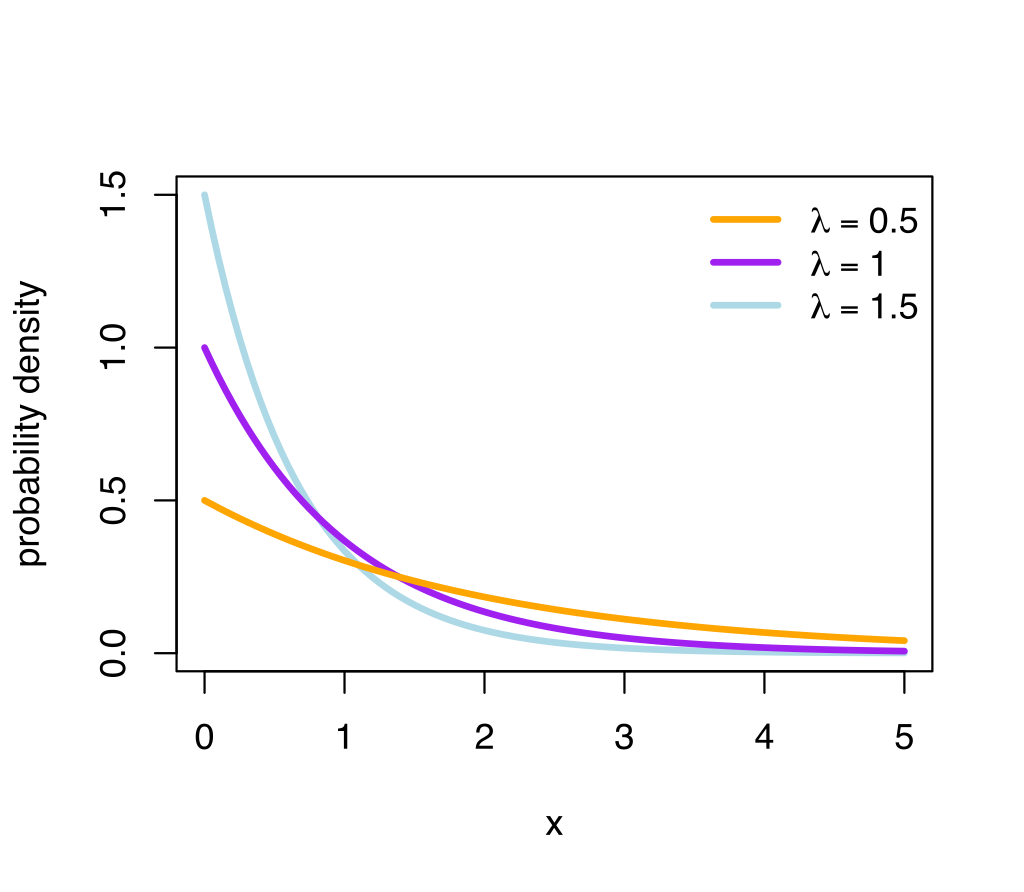
\includegraphics[scale=0.25]{plots/exponential.png}
    \caption{p.d.f. of Exponential distribution}
    \label{fig:exponential}
\end{figure}

\begin{remark}
The interpretation of Exponential distribution can be found via \href{https://www.probabilitycourse.com/chapter4/4_2_2_exponential.php}{Exponential distribution 1} and \href{https://www.statlect.com/probability-distributions/exponential-distribution}{Exponential distribution 2}. Pay attention to the connection between Exponential distribution and Poisson distribution.
\end{remark}
\end{example}

\begin{example}
\textbf{Normal (or Gaussian) distribution.} The most important continuous distribution, which has two parameters $\mu$ and $\sigma^2$ and density function
\begin{equation*}
    f(x) = \frac{1}{\sqrt{2\pi\sigma^2}} \exp \left( -\frac{(x-\mu)^2}{2\sigma^2} \right), \quad x\in\R. 
\end{equation*}
It is denoted by $N(\mu, \sigma^2)$. If $\mu=0$ and $\sigma^2=1$, then
\begin{equation*}
    f(x) = \frac{1}{\sqrt{2\pi}} e^{-\frac{1}{2}x^2}, \quad x\in\R.
\end{equation*}
is the density of the standard normal distribution. It is easy to generalize 2D case to multivariable case. Suppose $\mathbf{x} \in \R^n$, $\mathbf{\mu} \in \R^n$ is the mean vector and $\mathbf{\sigma}^2 \in \R^{n\times n}$ is the covariance matrix. Then
\begin{equation*}
    f(\mathbf{x}) = \frac{1}{\sqrt{(2\pi)^n} \det(\mathbf{\sigma}^2)} \exp \left( -\frac{1}{2} (\mathbf{x}-\mathbf{\mu})^T (\mathbf{\sigma}^2)^{-1} (\mathbf{x}-\mathbf{\mu}) \right), \quad \mathbf{x} \in \R^n.
\end{equation*}

\begin{remark}
For 2D case, if $\sigma^2$ is diagonal, then $f(x,y) = f(x)f(y)$. Therefore, $\sigma^2$ is a measure of independence. For multivariable cases, if $\sigma^2$ is diagonal, then all random variables are independent with each other.
\end{remark}
\end{example}


\end{document}